\chapter{Optimization}
\label{sec:opt}
Executing \textit{FloatingSE} by hand is sufficient to explore some simple
one-off or comparison analyses between a few runs.  OpenMDAO
provides extensive optimization capability, which can give yield richer
and more insightful analyses.  Beyond setting initial conditions for all
of the input variables, the user must also specify,
\begin{description}
\item[Design Variables]: The variables that are adjusted in order to
  find the optimal solution;
\item[Constraints]: The set of conditions that the solution must satisfy;
\item[Objective(s)]: The metrics used to minimize (or maximize) in the
  optimization problem; 
\item[Solver/Driver]: The algorithm used to find the optimal set of
  design variable values.
\end{description}

\section{Design Variables}
OpenMDAO currently only supports continuous design variables, those that
can take on any decimal value, because gradients with respect to the
objective function can be obtained.  Mixed-integer optimization drivers,
which can handle variables that take on discrete values (e.g. number of
mooring lines, or type of mooring line) are not yet fully implemented.
To realize the full analysis capabilities of \textit{FloatingSE}, an
mixed-integer optimization driver will have to be used.  Thus,
experimenting with this type of approach is in the near-term development
plan.

Aside from the restriction to continuous design variables, the user
could denote any variable as a design variable.  This is in fact a
feature of OpenMDAO, where any variable can be a design
variable, and any output could be a constraint or objective function.
The standard list of design variables in \textit{FloatingSE} given in
the examples are the continuous variables that parametrically describe
the geometry of the substructure listed in Section \ref{sec:geom}.  For
a succinct, central listing, these variables are collected together in
Table \ref{tbl:designvar}.

\begin{table}[htbp] \begin{center}
    \caption{Standard design variables used for optimization in \textit{FloatingSE}.}
    \label{tbl:designvar}
{\footnotesize
  \begin{tabularx}{\textwidth}{ l l c c X } \hline
    \textbf{Variable} & \textbf{Type} & \textbf{Units} & \textbf{Bounds} &\textbf{Description} \\ \hline \hline
    \mytt{base\_section\_height} & Float array ($n_s$) & $m$& 0.1--100&Height of each section \\
    \mytt{base\_outer\_diameter} & Float array ($n_s+1$) & $m$& 1.1--40&Diameter at each section node (linear lofting between)\\
    \mytt{base\_wall\_thickness} & Float array ($n_s+1$)  & $m$& 0.005--1&Wall thickness at each section node (linear lofting between) \\
    \mytt{base\_freeboard} & Float scalar & $m$&0--50 &Design height above waterline\\
    \mytt{base\_stiffener\_web\_height} & Float array ($n_s$) & $m$& 0.01--1&Stiffener web height for each section \\
    \mytt{base\_stiffener\_web\_thickness} & Float array ($n_s$) & $m$& 0.001--0.5&Stiffener web thickness for each section \\
    \mytt{base\_stiffener\_flange\_width} & Float array ($n_s$) & $m$& 0.01--5&Stiffener flange width for each section \\
    \mytt{base\_stiffener\_flange\_thickness} & Float array ($n_s$) & $m$& 0.001--0.5&Stiffener flange thickness for each section\\
    \mytt{base\_stiffener\_spacing} & Float array ($n_s$) & $m$& 0.01--10&Stiffener spacing for each section \\
    \mytt{auxiliary\_section\_height} & Float array ($n_s$) & $m$& 0.1--100&Height of each section \\
    \mytt{auxiliary\_outer\_diameter} & Float array ($n_s+1$)&$m$& 1.1--40&Diameter at each section node (linear lofting between)\\
    \mytt{auxiliary\_wall\_thickness} &Float array ($n_s+1$) &$m$& 0.005--1&Wall thickness at each section node (linear lofting between)\\
    \mytt{auxiliary\_freeboard} & Float scalar & $m$& 0--50 &Design height above waterline \\
    \mytt{auxiliary\_stiffener\_web\_height} & Float array ($n_s$) & $m$& 0.01--1&Stiffener web height for each section \\
    \mytt{auxiliary\_stiffener\_web\_thickness} & Float array ($n_s$) &$m$& 0.001--0.5&Stiffener web thickness for each section\\
    \mytt{auxiliary\_stiffener\_flange\_width} & Float array ($n_s$) &$m$& 0.01--5&Stiffener flange width for each section\\
    \mytt{auxiliary\_stiffener\_flange\_thickness} & Float array ($n_s$) &$m$& 0.001--0.5&Stiffener flange thickness for each section\\
    \mytt{auxiliary\_stiffener\_spacing} & Float array ($n_s$) & $m$& 0.01--10&SStiffener spacing for each section \\
    \mytt{radius\_to\_auxiliary\_column} & Float scalar &$m$& 0--40&Centerline of base column to centerline of auxiliary column\\
    \mytt{base\_permanent\_ballast\_height} & Float scalar & $m$& 0.1--50&Height above keel for permanent ballast \\
    \mytt{auxiliary\_permanent\_ballast\_height} & Float scalar & $m$& 0.1--50&Height above keel for permanent ballast \\
    \mytt{pontoon\_outer\_diameter} & Float scalar & $m$& 0.1--3&Diameter of all pontoon/truss elements \\
    \mytt{pontoon\_wall\_thickness} & Float scalar & $m$& 0.005--0.1&Thickness of all pontoon/truss elements \\
    \mytt{base\_pontoon\_attach\_lower} & Float scalar & $m$& -100--100&Lower z-coordinate on base where truss attaches \\
    \mytt{base\_pontoon\_attach\_upper} & Float scalar & $m$& -100--100&Upper z-coordinate on base where truss attaches \\
    \mytt{mooring\_diameter} & Float scalar & $m$& 0.05--1&Diameter of mooring line/chain \\
    \mytt{fairlead} & Float scalar & $m$& 0--200&Distance below waterline for attachment \\
    \mytt{fairlead\_offset\_from\_shell} & Float scalar & $m$ & 0--5& Offset from shell surface for mooring attachment \\
    \mytt{scope\_ratio} & Float scalar && 1--5&Ratio of line length to distance to sea floor (from fairlead)\\
    \mytt{anchor\_radius} & Float scalar & $m$& 1--1000&Distance from centerline to sea floor landing \\
  \hline \end{tabularx}
}
\end{center} \end{table}


\section{Constraints}
Due to the many design variables, permutations of settings, and applied
physics, there are many constraints that must be applied for an
optimization to close.  These constraints can be tuned with user inputs
and/or user-defined limits for the constraints in the optimization
problem set-up.  The constraints are described in detail in the
following sub-sections.  For convenience, all of the constraints, and
their bounds, are also collected together in Table \ref{tbl:constraints}.

\begin{table}[htbp] \begin{center}
    \caption{Optimization constraints used in \textit{FloatingSE}.}
    \label{tbl:constraints}
    {\footnotesize
  \begin{tabular}{ r l l |c| r l l} \hline
    \textbf{Lower} & \textbf{Constraint} & \textbf{Upper} && \textbf{Lower} & \textbf{Constraint} & \textbf{Upper} \\ \hline \hline
& \mytt{base.draft\_depth\_ratio} & $0.75$ && $1.0$ & \mytt{base.flange\_compactness} &\\
& \mytt{aux.draft\_depth\_ratio} & $0.75$&& $1.0$ & \mytt{base.web\_compactness} &\\
& \mytt{aux.fairlead\_draft\_ratio} & $1.0$&& $1.0$ & \mytt{aux.flange\_compactness} &\\
& \mytt{so.base\_auxiliary\_spacing} & $1.0$&& $1.0$ & \mytt{aux.web\_compactness} &\\
$\unit[0.0]{m}$ & \mytt{sg.transition\_buffer} & $\unit[2.0]{m}$&& & \mytt{base.axial\_local\_unity} & $1.0$\\
& \mytt{base.flange\_spacing\_ratio} & $1.0$&& & \mytt{base.axial\_general\_unity} & $1.0$\\ 
& \mytt{base.web\_radius\_ratio} & $1.0$&& & \mytt{base.external\_local\_unity} & $1.0$\\
& \mytt{aux.flange\_spacing\_ratio} & $1.0$&& & \mytt{base.external\_general\_unity} & $1.0$\\
& \mytt{aux.web\_radius\_ratio} & $1.0$&& & \mytt{aux.axial\_local\_unity} & $1.0$\\
$0.0$ & \mytt{load.pontoon\_base\_attach\_lower} & $0.5$&& & \mytt{aux.axial\_general\_unity} & $1.0$\\
$0.5$ & \mytt{load.pontoon\_base\_attach\_upper} & $1.0$&& & \mytt{aux.external\_local\_unity} & $1.0$\\
$1.0$ & \mytt{mm.mooring\_length\_min} &&& & \mytt{aux.external\_general\_unity} & $1.0$\\ 
& \mytt{mm.mooring\_length\_max} & $1.0$&& & \mytt{load.pontoon\_stress} & $1.0$\\
& \mytt{base.manufacturability} & $0.0$&& & \mytt{load.tower\_stress} & $1.0$\\ 
& \mytt{base.weldability} & $0.0$&& & \mytt{load.tower\_shell\_buckling} & $1.0$\\
& \mytt{aux.manufacturability} & $0.0$&& & \mytt{load.tower\_global\_buckling} & $1.0$\\
& \mytt{aux.weldability} & $0.0$&& $0.0$ & \mytt{mm.axial\_unity} & $1.0$\\
& \mytt{tow.manufacturability} & $0.0$&& $0.0$ & \mytt{sm.variable\_ballast\_height\_ratio} & $1.0$\\
& \mytt{tow.weldability} & $0.0$&& $0.0$ & \mytt{sm.variable\_ballast\_mass} &\\
$0.0$ & \mytt{load.base\_connection\_ratio} &&& $0.1$ & \mytt{sm.metacentric\_height} &\\
$0.5$ & \mytt{load.auxiliary\_connection\_ratio} &&& & \mytt{sm.offset\_force\_ratio} & $1.0$\\
&&&& & \mytt{sm.heel\_moment\_ratio} & $1.0$\\
    \hline \end{tabular}
  }
\end{center} \end{table}

\subsection{Geometry Constraints}
The user inputs the desired freeboard, fairlead, sea level depth, column
spacing, and initial section heights of the submerged columns.  The
constraints that ensures that the draft of the submerged columns does
not approach the water depth are,
\begin{lstlisting}
base.draft_depth_ratio $\leq$ 0.75
aux.draft_depth_ratio $\leq$ 0.75
\end{lstlisting}
where the prefixes, \texttt{base} and \texttt{aux}, have the same
meaning as in Table \ref{sec:exec}.  The 75\% value is up to the
user's discretion.

The fairlead attachment point of the moorings much also be less than the
draft of the column.  This is handled by,
\begin{lstlisting}
aux.fairlead_draft_ratio $\leq$ 1.0
\end{lstlisting}

If there are multiple submerged columns, the user specifies their radial
distance from the center of the structure and the diameters of all
columns.  A constraint to ensure that the outer shells of adjacent
columns do not intersect must be therefore be applied,
\begin{lstlisting}
sg.base_auxiliary_spacing $\leq$ 1.0
\end{lstlisting}

At the interface of the substructure and turbine tower, there must be a
platform for human access to the interface and tower internals.  This is
enforced by setting the difference between the substructure radius at
the tower interface and the tower radius at the base (in meters),
\begin{lstlisting}
$\unit[0.0]{m} \leq$ sg.transition_buffer $\leq \unit[2.0]{m}$
\end{lstlisting}

For submerged columns with ring stiffeners, the geometry must be
constrained such that the stiffener web is not greater than the column
radius and the stiffener flange is not greater than the half-spacing
between stiffeners.  These bounds are expressed as ratios that must be
less than one,
\begin{lstlisting}
base.flange_spacing_ratio $\leq$ 1.0
base.web_radius_ratio $\leq$ 1.0
aux.flange_spacing_ratio $\leq$ 1.0
aux.web_radius_ratio $\leq$ 1.0
\end{lstlisting}

Two of the possible design variables open to optimization are the
connection points of semisubmersible pontoons to the columns.  The
pontoon elements are classified as \textit{upper}, \textit{lower}, or
\textit{cross} (which connects an ``upper'' region to a ``lower'' one).
The upper and lower connection points can be adjusted by the
optimization, but constraints exist to ensure that they remain in the
upper or lower half, respectively, of the attaching columns,
\begin{lstlisting}
0.0 $\leq$ load.pontoon_base_attach_lower $\leq$ 0.5
0.5 $\leq$ load.pontoon_base_attach_upper $\leq$ 1.0
\end{lstlisting}

For the mooring lines, the user specifies the scope ratio (the ratio
between the total line length and the distance from the fairlead
connection to the sea floor) and the distance to the anchor site.
Constraints are needed to ensure there is sufficient line length to
reach the anchor site, but not so much line that there is no catenary
``hang'' and the line pools on itself on the sea floor.  These two
bounds are imposed with,
\begin{lstlisting}
mm.mooring_length_min $\geq$ 1.0
mm.mooring_length_max $\leq$ 1.0
\end{lstlisting}


\subsection{Manufacturing Constraints}
Manufacturing steel frustum shells requires rolling steel plates into
shape and welding along a seam to close the section.  To accommodate
traditional rolling and welding practices, both the diameter taper over
the course of a section and the wall thickness ratio relative to the
diameter are capped.  Similarly, to facilitate welding the
semisubmersible pontoons to the columns, constraints regarding the radio
of diameters between the two are enforced. These limits are determined
by user parameters in Table \ref{tbl:manconvar} and constraints,
\begin{lstlisting}
base.manufacturability $\leq$ 0.0
base.weldability $\leq$ 0.0
aux.manufacturability $\leq$ 0.0
aux.weldability $\leq$ 0.0
tow.manufacturability $\leq$ 0.0
tow.weldability $\leq$ 0.0
load.base_connection_ratio $\geq$ 0.0
load.auxiliary_connection_ratio $\geq$ 0.0
\end{lstlisting}

\begin{table}[htbp] \begin{center}
    \caption{Constraint variables for the manufacturability in \textit{FloatingSE}.}
    \label{tbl:manconvar}
{\footnotesize
  \begin{tabular}{l l l } \hline
    \textbf{Variable} & \textbf{Type} & \textbf{Description} \\
    \mytt{min\_taper\_ratio} & Float scalar & For manufacturability of rolling steel\\
    \mytt{min\_diameter\_thickness\_ratio} & Float scalar & For weld-ability\\
    \mytt{connection\_ratio\_max} & Float scalar & For welding pontoons to columns\\
  \hline \end{tabular}
}
\end{center} \end{table}

\subsection{Stress Limits and Code Compliance}
The stress and buckling code compliance constraints are formulated as
utilization ratios (ratio of actual to maximum values), with a safety
factor, which must be less than one. The safety factor parameters are
listed in Table \ref{tbl:safetyvar}.

\begin{table}[htbp] \begin{center}
    \caption{Variables specifying the factors of safety within \textit{FloatingSE}.}
    \label{tbl:safetyvar}
{\footnotesize
  \begin{tabular}{ l l l } \hline
    \textbf{Variable} & \textbf{Type} & \textbf{Description} \\
    \mytt{gamma\_f} & Float scalar & Safety factor on loads\\
    \mytt{gamma\_b} & Float scalar & Safety factor on buckling\\
    \mytt{gamma\_m} & Float scalar & Safety factor on materials\\
    \mytt{gamma\_n} & Float scalar & Safety factor on consequence of failure\\
    \mytt{gamma\_fatigue} & Float scalar & Not currently used\\
  \hline \end{tabular}
}
\end{center} \end{table}

For the ring stiffeners, there are ``compactness'' utilizations that
compare the geometry to the Young's modulus and yeild stress,
\begin{lstlisting}
base.flange_compactness $\geq$ 1.0
base.web_compactness $\geq$ 1.0
aux.flange_compactness $\geq$ 1.0
aux.web_compactness $\geq$ 1.0
\end{lstlisting}

The API checks on axial loading and buckling are captured with,
\begin{lstlisting}
base.axial_local_unity $\leq$ 1.0
base.axial_general_unity $\leq$ 1.0
base.external_local_unity $\leq$ 1.0
base.external_general_unity $\leq$ 1.0
aux.axial_local_unity $\leq$ 1.0
aux.axial_general_unity $\leq$ 1.0
aux.external_local_unity $\leq$ 1.0
aux.external_general_unity $\leq$ 1.0
\end{lstlisting}

Stress limits are imposed via the von Mises stress criterion relative to
the yield stress and a factor of safety such that a utilization
constraint is formed.  This is applied to both the tower and the
individual pontoons in the substructure truss,
\begin{lstlisting}
load.pontoon_stress $\leq$ 1.0
load.tower_stress $\leq$ 1.0
\end{lstlisting}

The tower also has shell and global buckling bounds described above,
\begin{lstlisting}
load.tower_shell_buckling $\leq$ 1.0
load.tower_global_buckling $\leq$ 1.0
\end{lstlisting}

Similar to the von Mises stress limits, the mooring line tension is also
constrained relative to the breaking load (which is an empiral function of
the diameter) and a safety factor
\begin{lstlisting}
0.0 $\leq$ mm.axial_unity $\leq$ 1.0
\end{lstlisting}
            
\subsection{Stability}
Neutral buoyancy is checked by ensuring that the variable ballast mass
required is positive and that there is enough payload capacity within
the column to hold the water,
\begin{lstlisting}
0.0 $\leq$ sm.variable_ballast_height_ratio $\leq$ 1.0
sm.variable_ballast_mass $\geq$ 0.0
\end{lstlisting}

Static stability is enforced by constraining the metacentric height to
be positive,
\begin{lstlisting}
sm.metacentric_height $\geq$ 0.1
\end{lstlisting}

As described above, surge and pitch stability are enforced through
similar approaches.  The total force and moment acting on the turbine
are compared to the restoring forces and moments applied by the mooring
system, buoyancy, or other sources at the maximum allowable point of
displacement.  These constraints are formulated as ratios with the user
specifying the maximum allowable limits via the variables in Table
\ref{tbl:moorcon}.
\begin{lstlisting}
sm.offset_force_ratio $\leq$ 1.0
sm.heel_moment_ratio $\leq$ 1.0
\end{lstlisting}

\begin{table}[htbp] \begin{center}
    \caption{Constraint variables for the mooring system in \textit{FloatingSE}.}
    \label{tbl:moorcon}
{\footnotesize
  \begin{tabular}{ l l c l } \hline
    \textbf{Variable} & \textbf{Type} & \textbf{Units} & \textbf{Description} \\
    \mytt{mooring\_max\_offset} & Float scalar & $m$& Max surge/sway offset \\
    \mytt{mooring\_max\_heel}   & Float scalar & $deg$& Max heel (pitching) angle \\
  \hline \end{tabular}
}
\end{center} \end{table}

\section{Objectives}
Different anaylses will emphasize different metrics, requiring different
objective functions.  Under the default assumption that the user wishes
to minimize cost and adhere to stability constraints, the objective
function would be total substructure cost (variable name,
\texttt{total\_cost}) or mass (variable name, \texttt{total\_mass}).

\section{Example}

\begin{figure}[htb]
  \begin{subfigure}[b]{0.49\linewidth}
    \centering 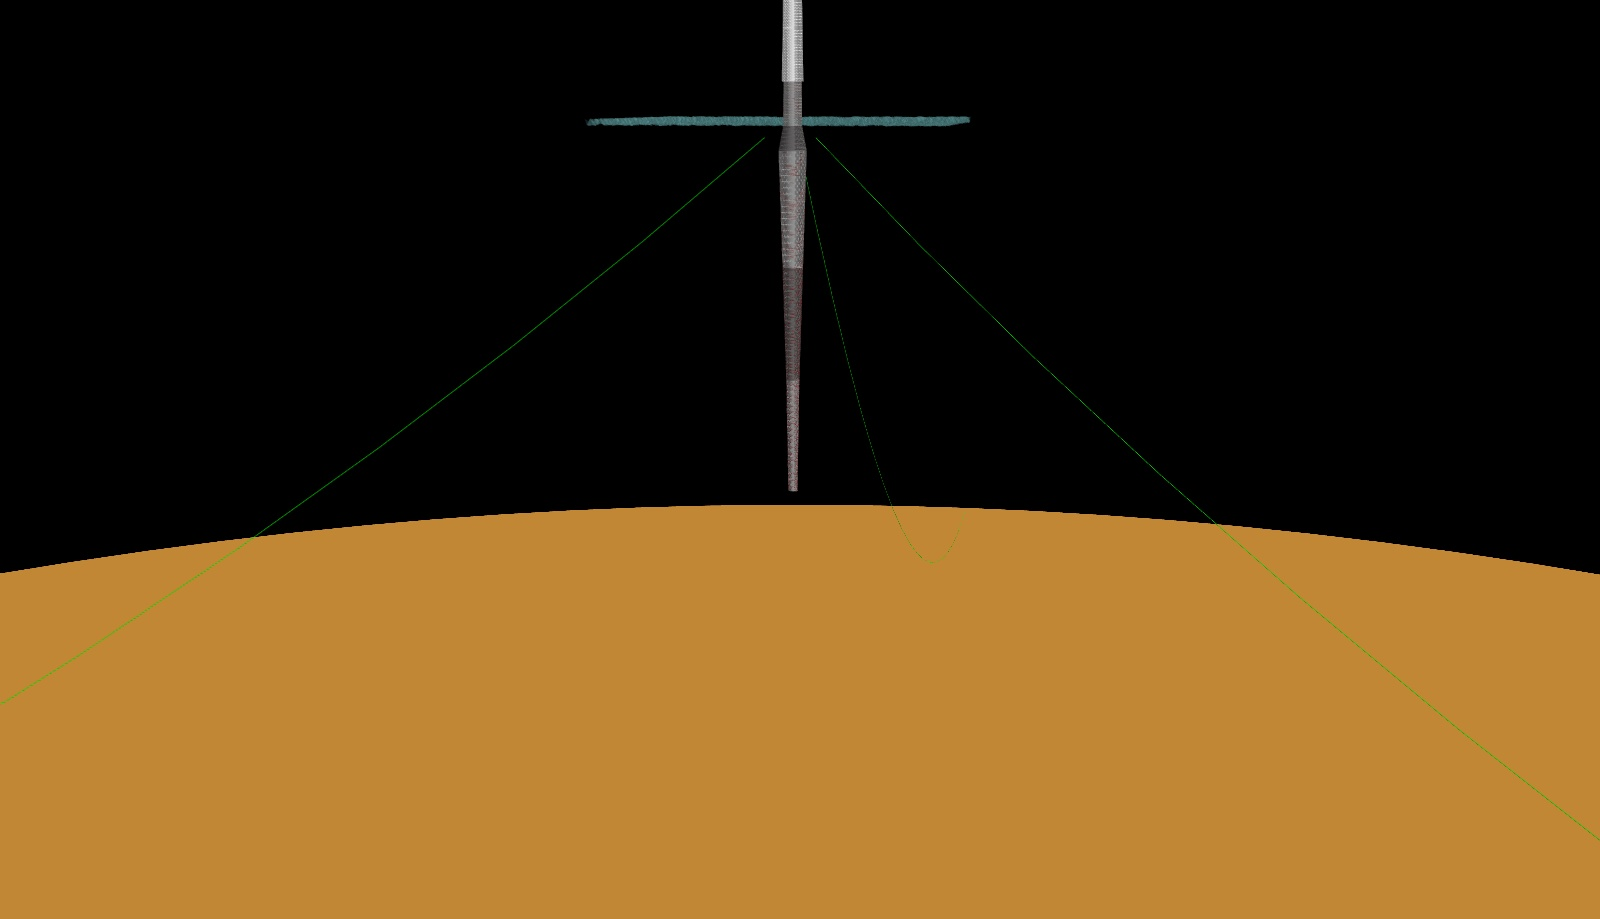
\includegraphics[width=\linewidth]{figs/spar-psqp.jpg}
    \caption{Spar}
  \end{subfigure}
  \begin{subfigure}[b]{0.49\linewidth}
    \centering 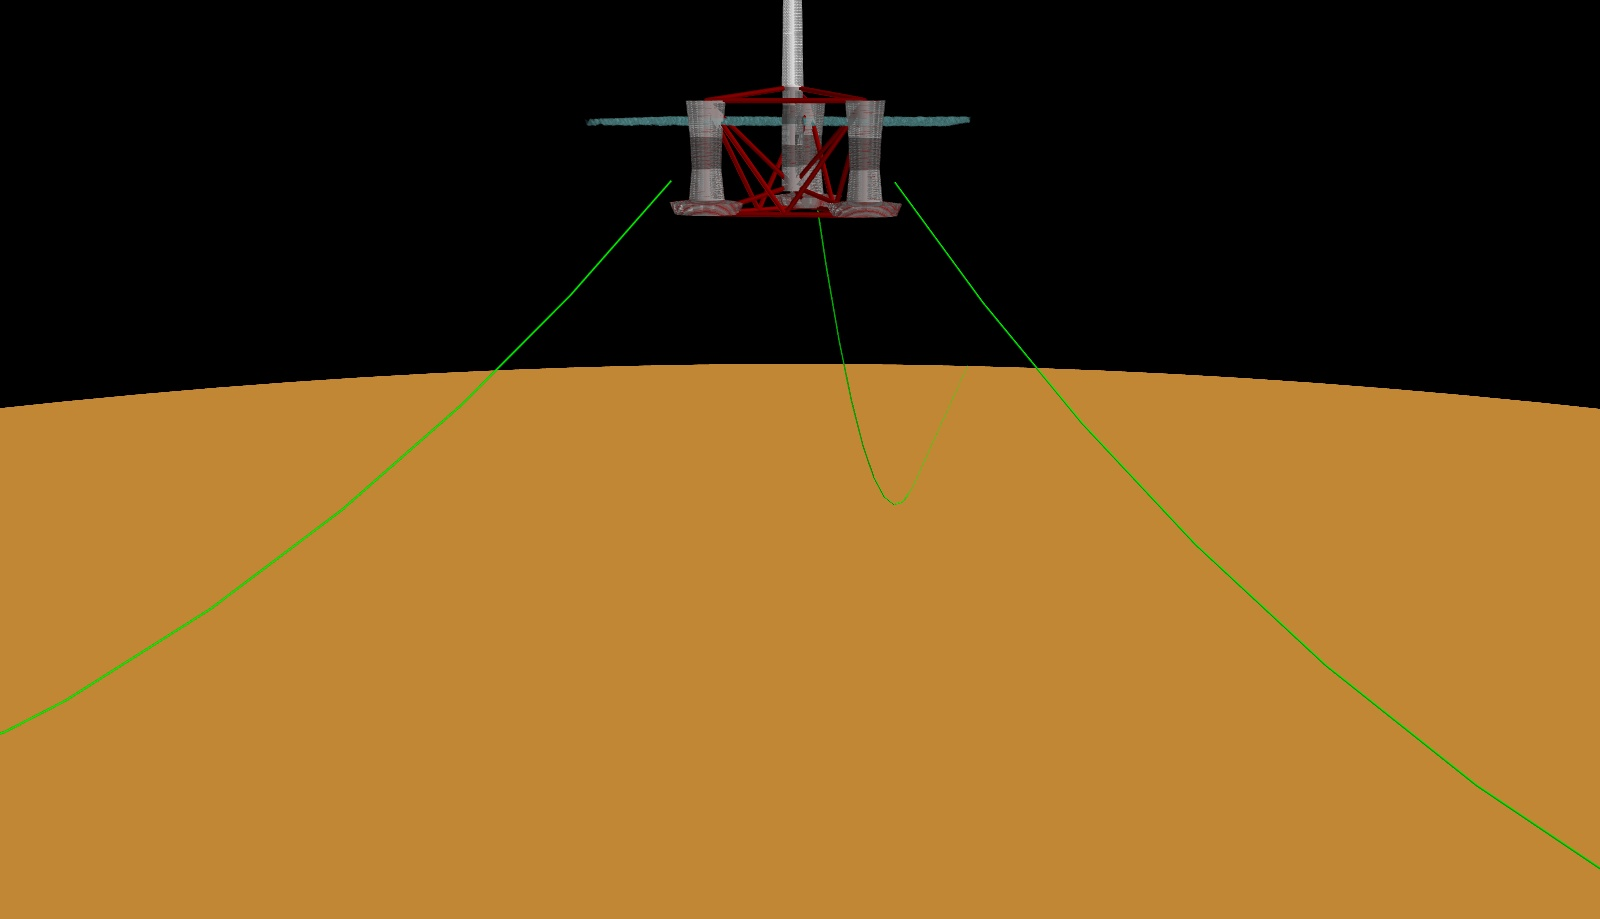
\includegraphics[width=\linewidth]{figs/semi-psqp.jpg}
    \caption{Semisubmersible}
  \end{subfigure}\\
  \caption{Examples of optimized spar and semisubmersible geometries.}
  \label{fig:optex}
\end{figure}

